% !TEX TS-program = XeLaTeX
% !TEX encoding = UTF-8 Unicode

\chapter{系统相关技术}
\label{系统相关技术}
\defaultfont

\section{Spring Boot介绍}

Spring Boot可以更快创建独立的、基于Spring的生产级应用。该框架解决了Spring框架配置非常烦琐的问题(Spring框架是轻量级的,但是它的配置却是重量级的),简化了项目开发流程\cite{.2019f}。

Spring Boot特点介绍(基于 Spring Boot 2.4.5 )

\begin{enumerate}
  \item 创建独立的Spring应用程序。
  \item 直接嵌入Tomcat、Jetty或Undertow(不需要部署WAR文件)。
  \item 提供可选择的“启动器”依赖项来简化构建配置。
  \item 尽可能地自动配置Spring和第三方库。
  \item 提供生产就绪特性,如度量、运行状况检查和外部化配置。
  \item 绝对不需要代码生成,也不需要XML配置。
\end{enumerate}

Spring Boot首次发布于2014年中期,为Spring生态系统带来了一种“opinionated”的方法,经过了很多的开发和改进。它的2.0版在2018年初发布。 在语言方面,Spring 5和Spring Boot 2需要Java 8,这使得使用核心Java 8函数成为可能。这包括接口上的默认方法和一些abstractxxxconfiguration类、Nullable-Support等相关的弃用。同时,Spring中使用的所有Java EE规范都升级到了Java EE 7。Spring Boot 1是支持Java 7的最后一个Spring Boot版本,而Spring Boot 2将是第一个运行在Java 9上的版本(预计也将运行在Java 10上),其中这还伴随着一些基本依赖项的升级:例如Tomcat、Hibernate和Gradle。

Spring Boot 2的一个亮点是几乎自动可用的HTTP/2支持:Tomcat、Jetty、Undertow和Reactor Netty的使用版本支持HTTP/2开箱即用。配置非常简单:服务器证书必须配置server.ssl.*下的属性。那么HTTP/2可以通过server.http2.enabled激活。HTTP/2是快速网络的重要构建块。可以通过压缩头、服务器推送、请求管道和多路复用请求来大幅降低延迟。

\subsection{Spring 5: Spring Boot 2及其模块的基础}

Spring出现于2003年,是为了应对早期J2EE规范的复杂性。虽然有些人认为Java EE和Spring是竞争对手,但Spring实际上是Java EE的补充。Spring编程模型不包含Java EE平台规范,相反,它与EE中精心挑选的各个规范集成在一起:

\begin{enumerate}
  \item Servlet API (JSR 340)
  \item WebSocket API (JSR 356)
  \item Concurrency Utilities (JSR 236)
  \item JSON Binding API (JSR 367)
  \item Bean Validation (JSR 303)
  \item JPA (JSR 338)
  \item JMS (JSR 914)
  \item 以及JTA/JCA设置,以便在必要时进行事务协调。
\end{enumerate}

Spring框架还支持依赖注入(JSR 330)和公共注解(JSR 250)规范,应用程序开发人员可以选择使用这些规范来代替Spring框架提供的特定于Spring的机制。

随着时间的推移,Java EE在应用程序开发中的角色已经演变。在Java EE和Spring的早期,创建应用程序是为了部署到应用服务器上。如今,在Spring Boot的帮助下,应用程序以一种对devops和云友好的方式创建,其中嵌入了Servlet容器,更改起来很简单。从Spring Framework 5开始,WebFlux应用程序甚至不直接使用Servlet API,可以运行在不是Servlet容器的服务器上(比如Netty)。

随着Spring框架的不断发展,第五代Spring框架于2017年9月底发布。Spring 5是Spring Boot 2 中的大多数框架的基础,并为“响应式编程”主题创建了基础。

Spring特点:

(1) Spring使创建Java企业应用程序变得很容易。它提供了在企业环境中使用Java语言所需的一切,支持Groovy和Kotlin作为JVM上的替代语言,以及根据应用程序的需要创建多种体系结构的灵活性。从Spring Framework 5.1开始,Spring需要JDK 8+(Java SE 8+),并提供对JDK 11 LTS的开箱即用支持。

(2) Spring支持广泛的应用程序场景。在大型企业中,应用程序往往存在很长时间,必须运行在JDK和应用服务器上,而JDK和应用服务器的升级周期超出了开发人员的控制范围。其他的可能作为一个内置服务器的jar运行,可能在云环境中。还有一些可能是不需要服务器的独立应用程序(如批处理或集成工作负载)。

(3) Spring是开源的。它有一个庞大而活跃的社区,基于各种不同的现实世界用例提供持续的反馈。这帮助Spring在很长一段时间内成功地发展。


\section{Spring Security介绍}

Spring Security是一个功能强大且高度可定制的身份验证和访问控制框架。它是保护基于spring的应用程序的实际标准。
目前比较流行的框架有两个,一个是Spring Security,另一个是Shiro。Shiro更加简单易用,Spring Security更容易和Spring整合,
更适应分布式应用,但是配置繁琐,概念复杂。近年随着Spring Boot的大火,Spring Security逐渐流行,因为前者在一定程度上简化了后者的配置。

Spring Security特点介绍(基于 Spring Security 5.5.0):
\begin{enumerate}
  \item 对身份验证和授权的全面且可扩展的支持。
  \item 防止例如点击劫持,跨站点请求伪造等攻击。
  \item Servlet API的集成。
  \item 与Spring Web MVC的可选继承。
\end{enumerate}

\subsection{Spring Security 5.5 新特性}

(1) OAuth 2.0 客户端

\begin{enumerate}[label=\circled{\arabic*}]
  \item 添加了对 Jwt客户端认证中的 private-key-jwt 和 client-secret-jwt 的支持。
  \item 添加了 Jwt Bearer Authorization Grant的支持。
  \item 增加了 ReactiveOAuth2AuthorizedClientService 的 R2DBC 实现。
\end{enumerate}

(2) OAuth 2.0 资源服务

\begin{enumerate}[label=\circled{\arabic*}]
  \item 增强的JWT译码器派生的签名算法
  \item 改进的内容协商
  \item 改进的 mult-tenancy 支持
\end{enumerate}

(3) SAML 2.0服务提供者

\begin{enumerate}[label=\circled{\arabic*}]
  \item 增加了OpenSAML 4的支持
  \item 增强的SAML 2.0断言解密
  \item 增加了基于文件的配置,用于断言当事人元数据
  \item 增强的依赖方元数据支持
  \item 增加了对ap-specified签名方法的支持
\end{enumerate}

(4) 配置

\begin{enumerate}[label=\circled{\arabic*}]
  \item 引入了DispatcherType请求匹配器
  \item 为过滤器安全性引入了AuthorizationManager
\end{enumerate}

(5) Kotlin DSL

\begin{enumerate}[label=\circled{\arabic*}]
  \item 添加rememberMe支持
\end{enumerate}

JSON Web Token(JWT)是一种开放的、行业标准RFC 7519方法,用于在双方之间安全地表示声明。如图\ref{jwt}是一个编码和解码的例子。
\begin{figure}[htbp]
  \centering
  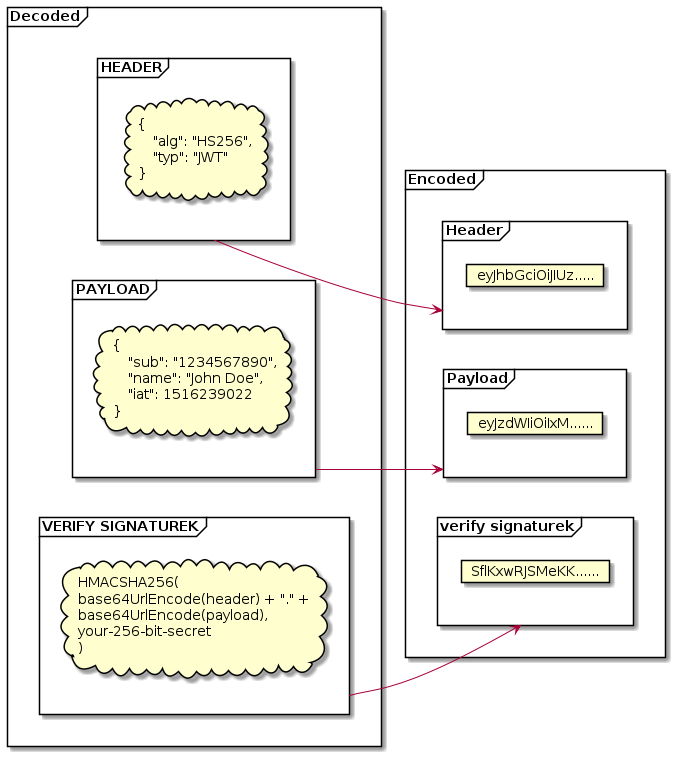
\includegraphics[scale = 0.55]{out/uml/部署图/JWT/JWT.png}
  \caption{\song\wuhao JWT示例}
  \label{jwt}
\end{figure}

\section{Spring Data Jpa 与 Hibernate介绍}

该介绍基于 Spring Data Jpa 2.5.1,Hibernate 5.4。目前主流的ORM(Object/Relation Mapping)工具有Hibernate和MyBatis。JPA、Spring Data JPA 和 Hibernate三者之间的关系:

(1) JPA

JPA(Java Persistence API)为对象-关系(ORM)映射提供了POJO持久性模型。JPA是一种规范,仅定义了接口,但是并没有实现。

(2) Spring Data JPA

Spring Data Jpa 是 Spring Data 的一部分,该模块着力于对基于JPA的数据访问层进行增强,简单的说它是一个简化Jpa的框架。很长一段时间以来,实现应用程序的数据访问层一直很费事,为了执行简单的查询以及分页和审计,必须编写太多的模板代码,而Spring Data Jpa可以通过编写接口自动生成sql,由框架完成复杂且重复的工作,减少了开发人员许多不必要的工作量。同时该框架可以使用面向对象的查询方式取代直接编写SQL语句也使代码更容易调试和查找bug。

Spring Data Jpa特点:
\begin{enumerate}[label=\circled{\arabic*}]
  \item 很好的构建基于Spring和Jpa的存储库。
  \item 支持Querydsl谓词,从而支持类型安全的JPA差选。
  \item 对于领域类有选择的映射属性。
  \item 分页支持,动态查询支持,集成自定义数据访问代码。
\end{enumerate}

(3) Hibernate

Hibernate是实现了JPA规范的框架(图\ref{JpaAndHibernate})。
\begin{figure}[htbp]
  \centering
  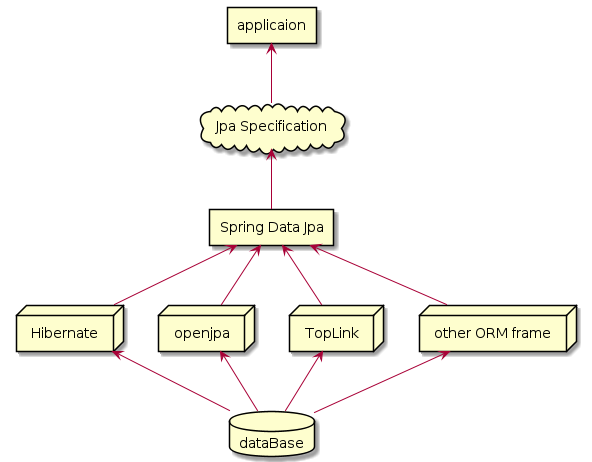
\includegraphics[scale = 0.5]{out/uml/部署图/Jpa和Hibernate/Jpa和Hibernate.png}
  \caption{\song\wuhao Jpa和Hibernate}
  \label{JpaAndHibernate}
\end{figure} Hibernate与MyBatis之间的对比和Spring Security与Shiro的对比很相似,使用Hibernate可以在完全不写SQL语句的情况下实现数据库操作,在写好配置之后,基于面向对象的查询方式让代码更简洁,易移植,易复用,减少了许多工作量,避免了许多因查询语句造成的差错,但是随着需求的增多即查询变得更加复杂,需要对框架有更好的理解才能才能编写出无差错的查询。

Hibernate特点:
\begin{enumerate}[label=\circled{\arabic*}]
  \item Hibernate有自己的原生API,但最为JPA标准的实现,它可以在任何支持JPA的环境中使用,包括括Java SE应用程序,Java EE应用程序服务器,Enterprise OSGi容器等。
  \item 允许按照自然的面向对象的方式进行持久化开发。Hibernate不需要持久化的接口或基类,并且允许任何类或数据持久化。
  \item Hibernate具有较高的性能,它支持延迟初始化,大量的抓取策略和带有自动版本控制和时间戳的乐观锁。无论是开发人员生产方面还是在运行时性能方面,它始终拥有优于直接使用JDBC代码的性能。
  \item Hibernate被设计为在应用服务器集群中工作,并提供高度可伸缩的体系结构。它在任何环境中都可以很好地扩展:不论是运行在内部网的低并发应用程序(只服务于几百个用户)还是运行在互联网上的高并发应用程序(服务于数十万用户),Hibernate都可以很好的驱动。
  \item Hibernate拥有卓越的稳定性和质量。
\end{enumerate}

总的来说,Hibernate是一个很强大的ORM工具,但是如果想要使用好它,是需要较多的经验的。

\section{Vue.js介绍}

(1) Vue.js是轻量级框架

该框架可以快速下载和安装库。

(2) 虚拟 DOM 渲染及其性能

相关概念:
\begin{enumerate}[label=\circled{\arabic*}]
  \item DOM(The Document Object Model):Web页面的API,允许读取和操作页面的内容,结构和样式。一种对HTML基于对象的表示(HTML文档 $\leftrightarrow$ 对象模型)
  \item node tree:DOM的对象结构。
  \item Render Tree:(DOM:element的表示 + CSSOM:element样式的表示)
\end{enumerate}

虚拟DOM:如果对象更改了它的状态,浏览器需要更新信息并且重新渲染到屏幕上,这个过程需要更新所有的DOM,开销是很大的。而Vue.js利用虚拟DOM解决了这个问题,可以将虚拟DOM理解为DOM的一个拷贝并且它可以找到需要更新的element而不是直接更新所有的element,这大大地提高了应用程序的性能。

(3) 响应式的双向数据绑定(图\ref{tow-way-date-binding})

Vue 改变了前端开 发者使用 jQuery 直接对页面上的 DOM 元素进行操作 的习惯,通过数据和模板双向绑定的形式更好地组织和 简化了 Web 开发。\cite{.2020g}

\begin{figure}[htbp]
  \centering
  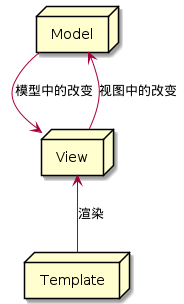
\includegraphics[scale = 0.6]{out/uml/部署图/Two-way data binding/Two-way data binding.png}
  \caption{\song\wuhao 双向数据绑定}
  \label{tow-way-date-binding}
\end{figure}

(4) CBA

Vue是基于组件的体系结构(Component Based Architecture(CBA)),这种体系结构的好处主要有:
\begin{enumerate}[label=\circled{\arabic*}]
  \item 代码的可读性:每个组件可以保存在同一个单独的文件,包括结构,样式和逻辑,可以通过代码看出这个组件的功能。
  \item 组件复用:封装好的组件可以在多个地方使用。
  \item 便于单元测试:每个组件刚好可以作为单元测试的一个单元。
\end{enumerate}

(5) Vue3变化
\begin{enumerate}[label=\circled{\arabic*}]
  \item 创建app的变化
        该改变解决了Vue2全局配置在单元测试中产生的问题(测试用户会因全局配置而互相影响)
  \item 多Root
        即可以去掉template中最外层的div。
  \item 组合式API。这应该是Vue3最大的变化,该变化主要是为了解决Vue2大组件难以阅读和维护的问题以及管理和维护组件之间的逻辑的问题。主要变化有:
        \begin{itemize}
          \item Setup

                代替 Vue2 中的 beforeCreate() 和 created()。

          \item Reactive References\\
                \lstinline[language = Java]| ref |即“Reactive References”,它包装了原始数据并且允许我们跟踪变化。(在Vue2中是使用\lstinline[language = Java]| data() |包装原始内部对象)
          \item Methods/Computed/Watch\\
                Vue2中有一个单独的methods/Computed/Watch部分用来编写方法,在vue3中则在setup()中编写。
          \item Props\\
                在Vue3中不需要this就可以访问props
          \item 移除了Vue filter\\
                在Vue2中filter主要用于普通文本的格式化,而在Vue3中被移除了。移除的主要原因是它的性能和普通的函数没有区别,而写成普通的函数则会有更大的复用空间。
          \item 多个v-model\\
                一个组件可以处理多个v-model,这样在多值处理的情况下,Vue3能更简单地通过多个event将值从子组件传递到父组件。
          \item 模块化\\
                可以将setup()中的内容分离到另一个composition function中并保存在一个js文件中以便重用。
          \item 声明周期钩子
                \begin{itemize}
                  \item (Vue2)beforeCreate()
                  \item (vue2)无$\Rightarrow$(Vue3)setup()
                  \item (Vue2)created()
                  \item (Vue2)beforeMount()
                  \item (Vue2)mounted()
                  \item (Vue2)beforeUpdate()
                  \item (Vue2)updated()
                  \item (Vue2)beforeDestroy()$\Rightarrow$(Vue3)beforeUnmount()
                  \item (Vue2)destroyed()$\Rightarrow$(Vue3)unmouted()
                  \item (Vue3)onRenderTracked()
                  \item (Vue3)onRenderTriggered()
                \end{itemize}
                并且beforeCreate()和create()不再需要,它们的工作放在setup()中完成。
        \end{itemize}
\end{enumerate}

\section{Vuex介绍}

Vuex是Vue.js应用程序的状态管理模式库。它作为应用程序中所有组件的集中存储,其规则确保状态只能以可预测的方式变化。它还集成了Vue的官方devtools扩展,以提供诸如零配置 time-travel 调试和状态快照导出/导入等高级特性。

\subsection{状态管理模式}

一个Vue app包括三个部分
\begin{enumerate}[label=\circled{\arabic*}]
  \item 状态(state),真正推动程序运行的源头。
  \item 视图(view),状态的声明性映射。
  \item 动作(actions),状态可能改变的方式,以响应用户从视图的输入。
\end{enumerate}

如图\ref{vuex-one-way-data-flow}是一个单向数据流的例子。

\begin{figure}[htbp]
  \centering
  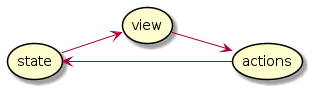
\includegraphics[scale = 0.6]{out/uml/部署图/vuex-one-way-data-flow/vuex-one-way-data-flow.png}
  \caption{\song\wuhao 单向数据流}
  \label{vuex-one-way-data-flow}
\end{figure}

当有多个共享同一个状态的组件时,不同组件之间需要传递装状态去同步状态,这个过程是复杂并且容易出错的。所以将状态从组件中提取出来统一管理,如图\ref{vuex-state-management-pattern}所示,任何组件都可以访问状态以及改变状态,从而免除了传递状态的过程。这种模式使代码更容易维护。

\begin{figure}[htbp]
  \centering
  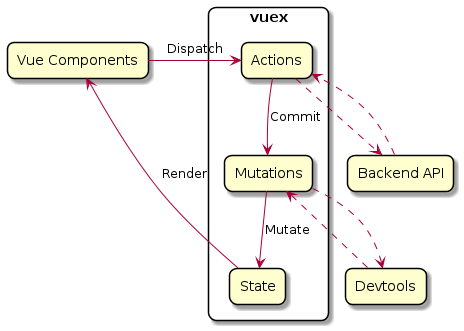
\includegraphics[scale = 0.5]{out/uml/部署图/vuex-state-management-pattern/vuex-state-management-pattern.png}
  \caption{\song\wuhao 状态管理模式}
  \label{vuex-state-management-pattern}
\end{figure}

五个核心概念:


(1) State

Vuex使用单一的状态树,这意味着每个应用程序都使用一个单一的状态树,但是这并不会与Vue的模块化思想冲突,因为Vuex同样可以将state、mutation和actions分割为各个子模块,使用namespace可以保证各个子模块中的state、mutation和actions可以使用和其他子模块重复的名字。

(2) Getters

Vuex允许在存储中定义“getter”。可以将它们视为存储的computed属性。与computed属性一样,getter的结果是基于它的依赖关系进行缓存的,并且只有在它的一些依赖关系发生变化时才会重新计算。

(3) Mutations

在Vuex~store中实际更改状态的唯一方法是提交一个mutation。Vuex~mutation与事件非常相似:每个mutation都有一个字符串类型和一个处理程序。

(4) Actions

Action和mutation相似,不同之处在于mutation操作state,action操作mutation,以及action可以使用异步操作。

(5) Modules

随着应用程序的增长,如果所有的状态都粗放在一个对象中,会变得非常臃肿,这时可以将其划分为许多子模块。

\section{Echarts介绍}

Echarts是快速构建基于web可视化的声明性框架,该框架的特点如下:

\begin{enumerate}
  \item 灵活的图表类型:Apache Echarts提供了20多种现成的图表类型,以及十几种组件,每个组件都一个任意组合使用。
  \item 优雅的视觉设计:默认设计遵循可视化原则,支持响应式设计。灵活的配置使其易于定制。
  \item 友好的可访问性:自动生成的图表描述帮助有阅读障碍的用户理解图表的内容和背后的故事。
  \item 强大的渲染引擎:可以轻松地切换画布和SVG渲染。渐进式渲染和流加载使实时渲染超大数据成为可能。
  \item 专业的数据分析:通过数据集管理数据,数据集支持数据转换,如过滤,类聚和回归,以帮助实现相同数据的多维分析。
  \item 一个健康的社区:活跃的开源社区确保了项目的健康发展,并为第三方扩展贡献了丰富的资源。
\end{enumerate}

\section{本章小结}

本章主要介绍了系统使用的相关技术,描述了其他类似的技术,介绍了选择这些技术的原因,在技术的选择上都考虑到了功能是否较为强大,社区是否较为活跃,扩展性是否较强等等,综合多方面进行考虑,为顺利实现一个稳定易扩展的系统打下基础。

% 删掉了 为之后顺利k